		Here, we analyze the efficiency of the  explicit Steklov method \eqref{Steklov} for
	SDEs for which a step size of the usual stochastic algorithms has to be  small  enough
	to preserve numerical stability. In particular, we consider as benchmarks the examples
	given in \cref{sec:SteklovMethod} to show the behavior of the Steklov scheme and compare it
	with the EM approximation, the CBD method \cite{Braanka1998} and a 
	balanced implicit method \cite{Schurz2007}. Moreover, long-time simulations of the new method
	are carried out in order to evidence  its good asymptotic dynamical properties.  But
	before, we start by evaluating the accuracy of the Steklov method for the linear SDE
	where the analytical solution is known.
	\subsection{Linear SDE}
		We apply the explicit Steklov approximation to the multiplicative \eqref{SDE} and
		additive \eqref{SDEa} linear SDEs and study its accuracy showing its strong error
		which is determined by
		\begin{equation}\label{eqn:StrongError}
			\varepsilon=\mathbb{E}
			\left(
				|y(T)-Y_{n_T}|
			\right),
		\end{equation}
		where  $y(t)$ is the exact solution  and  $Y_n$ is a time discretization approximation
		for the linear SDEs. Moreover, we also present numerical results for the
		EM scheme  for the same equations. Numerical  results for the Steklov
		and Euler-Maruyama (EM) approximations for both additive and multiplicative cases are
		shown in tables \ref{t1} and \ref{t2} respectively. The confidence interval for the
		strong error is obtained for $20$ samples of $100$ trajectories each. We also
		estimate the mean square error at a discrete time $t_n=T$ as follows:
		\begin{align}\label{eqn:MSEerrort}
			\varepsilon_{MS}(T)
			&=
			\left(
			\frac{1}{N}\sum_{k=1}^{N}
				\left(
					y^{[k]}(T)-Y_{n_T,k}^{h}
				\right)^2
			\right)^{\frac{1}{2}}, 
		\end{align}
		for $N=\num{100000}$ paths. Table \ref{t3} shows the results for both Steklov and
		Euler-Maruyama schemes. Notice that the Steklov method  maintains its accuracy even
		when the step size is close to one while the Euler-Maruyama approximation is no longer
		stable from $h=\num{0.5}$.
 \begin{table}[h!] 
    \centering
    \begin{tabular}{lll}
	\toprule
	\multicolumn{1}{c}{$h$}	&\multicolumn{1}{c}{EM}	&\multicolumn{1}{c}{Steklov}\\
	\midrule
	\num{0.25000}	&\num{4.1463e-02}$\pm$\num{2.9553e-03}	&\num{4.1076e-02}$\pm$\num{2.5145e-03}\\
	\num{0.50000}	&\num{1.2815e+02}$\pm$\num{1.3437e-01}	&\num{5.5109e-02}$\pm$\num{3.6455e-03}\\
	\num{0.75000}	&\num{7.8644e+02}$\pm$\num{5.9516e-01}	&\num{6.8446e-02}$\pm$\num{3.7039e-03}\\
	\num{1.00000}	&\num{1.2800e+03}$\pm$\num{5.7282e-01}	&\num{7.8523e-02}$\pm$\num{6.0528e-03}\\
	\bottomrule
    \end{tabular}
    \caption{Intervals at $\num{95}$\% of confidence of the strong error 
    for the additive  linear SDE  with 
    $\lambda=-5$, $\xi=\num{0.1}$ and initial condition $x_0=5$. } \label{t1}
 \end{table}
\begin{table}[h!]
    \begin{center}
      \begin{tabular}{ccc}
	\toprule
	$h$	&EM	&Steklov\\
	\midrule
	\num{0.12500}	&\num{1.8376e-02}$\pm$\num{8.3217e-04}	&\num{1.8376e-02}$\pm$\num{8.3217e-04}\\
	\num{0.25000}	&\num{1.7452e-02}$\pm$\num{1.3495e-03}	&\num{1.7452e-02}$\pm$\num{1.3495e-03}\\
	\num{0.50000}	&\num{1.2824e+02}$\pm$\num{1.4210e+00}	&\num{1.7774e-02}$\pm$\num{1.3205e-03}\\
	\bottomrule
      \end{tabular}
    \end{center}
    \caption{
      Intervals at $\num{95}$\% of confidence of the strong error for the multiplicative
      linear SDE  with $\lambda=-5.0$,  $\xi=\num{0.1}$ and  initial condition
      $x_0=5$.}\label{t2}
\end{table}
 \begin{table}[h!]
    \centering
    \begin{tabular}{lllll}
	\toprule
      &\multicolumn{2}{c}{Additive noise}
      &\multicolumn{2}{c}{Multiplicative noise}\\
      \cmidrule(r){2-3}
      \cmidrule(r){4-5}\\
      \multicolumn{1}{c}{$h$}	&\multicolumn{1}{c}{EM}
      &\multicolumn{1}{c}{Steklov}	&\multicolumn{1}{c}{EM}	&\multicolumn{1}{c}{Steklov}\\
      \cmidrule(r){2-2}		\cmidrule(r){3-3}
      \cmidrule(r){4-4}		\cmidrule(r){5-5}\\
	\num{0.2500}	&\num{2.1300e-01}		&\num{2.0367e-01} 		&\num{5.4261e-03}		
&\num{9.4396e-07}\\	
	\num{0.5000}	&\num{3.5206e+02}		&\num{3.0370e-01} 		&\num{2.7560e+02}		
&\num{1.0752e-03}\\
	\num{0.7500}	&\num{8.1368e+02}		&\num{3.9055e-01} 		&\num{8.5490e+02}		
&\num{7.1843e-02}\\
	\num{1.0000}	&\num{1.2930e+03}		&\num{4.5875e-01} 		&\num{1.3337e+03}		
&\num{2.8987e-01}\\
	\bottomrule
    \end{tabular}
    \caption{MS-Error at  time $T=\num{4.0}$ for a linear SDE with 
    $\lambda=-5$,  $\xi=\num{0.1}$ and initial condition $x_0=5$.
    }\label{t3}
  \end{table} 
	\subsection{Logistic equation}
		Here we reconsider the stochastic logistic  equation \eqref{eqn:SDELogistic}
		\begin{equation*}
			dy(t)= \lambda y(t)(K-y(t))dt+ \xi y(t)^\alpha|K-y(t)|^\beta dW(t),
		\end{equation*}
		where $y(t)$  represents the number of individuals of certain specie with growth rate
		$\lambda$ into an environment with limited  natural resources and $K$ is the maximum
		capacity population; $\alpha$, $\beta$ and $\xi$ are nonnegative coefficients linked
		with the random contribution that models the influence of the environmental fluctuations
		or measurement errors \cite{Pasquali2001,Schurz2007,Sun2008}. The analytical solution of
		this equation in general is unknown. Thus it is necessary to obtain  numerical
		solutions. In order to get an accuracy approximation it is desirable that the stochastic
		numerical method  preserves the dynamic properties of the solution of
		\eqref{eqn:SDELogistic}. We choose this example to emphasize the structural dynamical
		consistency between the explicit Steklov defined by the function $\Psi_h$ \eqref{psi2}
		and the SDE \eqref{eqn:SDELogistic}. In figure \ref{fig:PathsEDELog}, we  
		show the numerical results of the  Steklov and Euler-Maruyama schemes and a
		balanced implicit method (BIM) developed to solve the equation \eqref{eqn:SDELogistic} in 
		\cite{Schurz2007}. For step sizes greater than $\num{0.01}$,
		we observe that the Euler scheme is outside of its stability region and the BIM method has
		a slow convergence. On the other hand,
		the Steklov preserves the deterministic solution profile which is consistent with its
		structural foundation.
		\begin{figure}[h!]
			\hspace*{-0.2cm}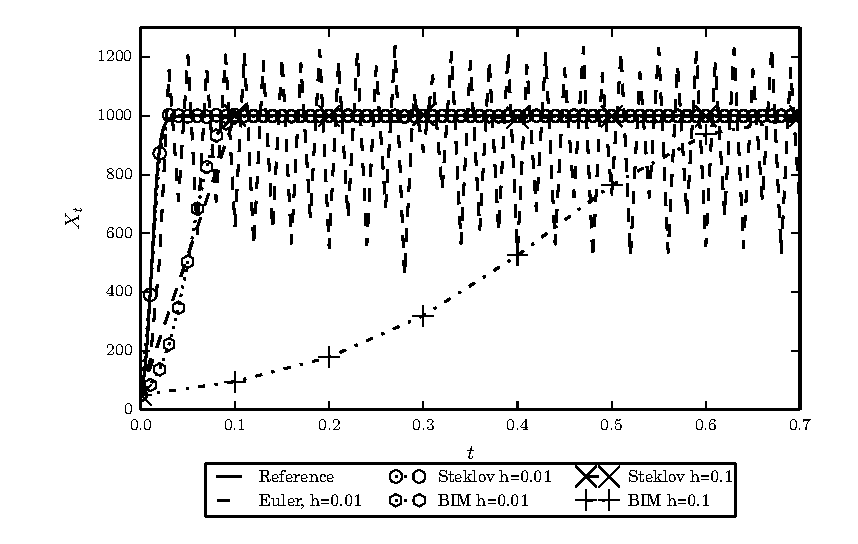
\includegraphics{./papers/paperA/figures/fig1.eps}
			\caption{
			Paths obtained with the Euler, Steklov and BIM methods for the logistic SDE 
			\eqref{eqn:SDELogistic} with $X_0=50$ and taking $K=1000$,
			$\alpha=1$, $\beta$=0.5, $\lambda$=0.25, $\rho=0$ and $\sigma$=$\num{0.05}$.%
			}\label{fig:PathsEDELog}%
		\end{figure}
	\subsection{Langevin equation in Brownian dynamics}\label{sec52}
	Finally, we study the Langevin equation (LE)
	\begin{equation*}
		dy(t)= -y(t)^3dt+
		\xi dW(t), 
	\end{equation*}
		where $y(t)$ is the position of a particle at time $t$ which is exposed to
	deterministic and random forces. This   equation is used in Brownian dynamics like a
	benchmark test, see \cite{Braanka1998}.  As in the logistic SDE, the analytical solution
	for the Langevin equation is only obtained under special conditions. The most common
	Brownian dynamics algorithm  is the CBD method of \citet*{Ermak1978}
	which is based on the Euler discretization of the LE. Although this method is easy to
	implement, a small time step size is required, therefore this algorithm  runs in
	relatively small temporal windows. So, to study the  asymptotic behavior of the solution
	of the LE it is convenient to apply methods with good asymptotic stability properties
	and simple structure. Therefore we show the behavior of the Steklov  method defined by
	the function \eqref{psi3} for short-time and long-time dynamics by  computing  the {\it
	self-diffusion} coefficient $D/D_0$ associated to the LE, for details of the derivation
	of this coefficient see  \cite{Braanka1998, Lowen1993}. In
	figure\ref{fig:PlotXcubicMSD}, we compare the profiles of the Steklov and
	CBD approximations for several step sizes. According to the notation in Brownian
	dynamics, we take Dta=0.00001 as time step size and use 10 000 sample paths to calculate
	the self-diffusion coefficient. The Steklov and  CBD methods have the same behavior at
	short time with small step sizes. However, for step sizes greater than 1 000 Dta the
	Euler method diverges and the Steklov method preserves its numerical stability. Thus, it
	can be used for long-time dynamics with  big step sizes as it is shown in  figure
	\ref{fig:PlotXcubicMSD}.
	\begin{figure}[h!]
		\begin{center}
			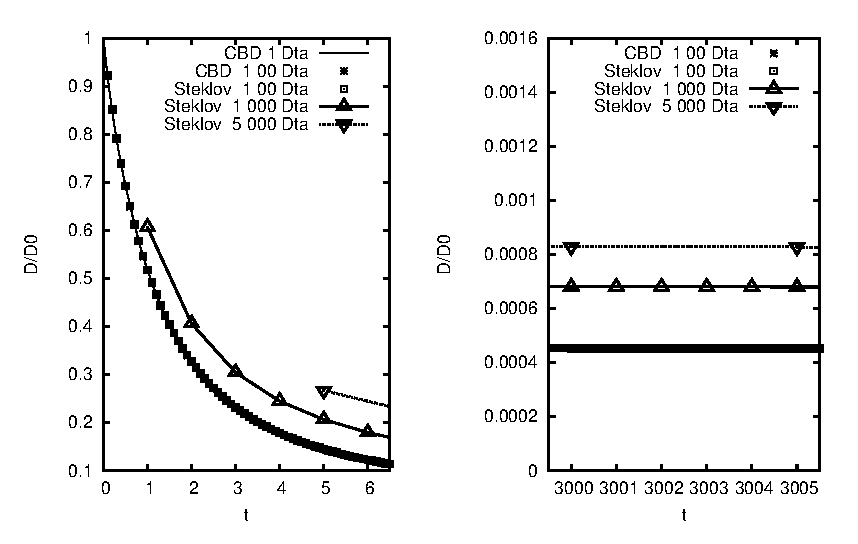
\includegraphics{./papers/paperA/figures/short-longMSD.eps}
		\end{center}
		\caption{
		Numerical results of the Steklov and CBD methods for the self-diffusion coefficient
		of the LE with $\xi=1$: the graph to the left shows short-time simulations and the
		graph to the right  shows long-time simulations. }\label{fig:PlotXcubicMSD}%
	\end{figure}
